%%%%%%%%%%%%%%%%%%%%%%%%%%%%%%%%%%%%%%%%%%%%%%%%%%%%%%%%%%%%%%%%%%%%%%%%%%%%%%%%
%2345678901234567890123456789012345678901234567890123456789012345678901234567890
%        1         2         3         4         5         6         7         8

\documentclass[letterpaper, 10 pt, conference]{ieeeconf}  % Comment this line out if you need a4paper

%\documentclass[a4paper, 10pt, conference]{ieeeconf}      % Use this line for a4 paper

\IEEEoverridecommandlockouts                              % This command is only needed if 
                                                          % you want to use the \thanks command

\overrideIEEEmargins                                      % Needed to meet printer requirements.

%In case you encounter the following error:
%Error 1010 The PDF file may be corrupt (unable to open PDF file) OR
%Error 1000 An error occurred while parsing a contents stream. Unable to analyze the PDF file.
%This is a known problem with pdfLaTeX conversion filter. The file cannot be opened with acrobat reader
%Please use one of the alternatives below to circumvent this error by uncommenting one or the other
%\pdfobjcompresslevel=0
%\pdfminorversion=4

% See the \addtolength command later in the file to balance the column lengths
% on the last page of the document

% The following packages can be found on http:\\www.ctan.org
\usepackage{graphics} % for pdf, bitmapped graphics files
%\usepackage{epsfig} % for postscript graphics files
%\usepackage{mathptmx} % assumes new font selection scheme installed
%\usepackage{times} % assumes new font selection scheme installed
\usepackage{amsmath} % assumes amsmath package installed
\usepackage{amssymb}  % assumes amsmath package installed

\title{\LARGE \bf
Union of Intersections (UoI) for Interpretable Data Driven Discovery and Prediction in Neuroscience
}


\author{
    Pratik S. Sachdeva$^{1}$ and Kristofer E. Bouchard$^{1,2*}$%
    \thanks{
        $^{1}$Redwood Center for Theoretical Neuroscience, UC Berkeley
    }%
    \thanks{
        $^{2}$Lawrence Berkeley National Laboratory
    }%
    \thanks{
        $^*$Corresponding author
    }%
}


\begin{document}



\maketitle
\thispagestyle{empty}
\pagestyle{empty}


%%%%%%%%%%%%%%%%%%%%%%%%%%%%%%%%%%%%%%%%%%%%%%%%%%%%%%%%%%%%%%%%%%%%%%%%%%%%%%%%
\begin{abstract}

Interpretable and predictive statistical data analysis methods can provide insight into the biological processes that generate neuroscience data.  However, commonly used statistical inference procedures generally fail to identify the correct features, and further introduce consequential bias in the estimates. To address these issues, we developed Union of Intersections (UoI), a flexible, modular, and scalable framework for enhanced statistical feature selection and estimation. Methods (e.g., regression, classification, dimensionality reduction) based on UoI perform feature selection and feature estimation through intersection and union operations, respectively. In the context of linear regression (specifically UoI$_{\text{Lasso}}$), we summarize extensive numerical investigation on synthetic data to demonstrate tight control of false-positives and false-negatives in feature selection with low-bias and low-variance estimates of selected parameters, while maintaining high-quality prediction accuracy (in the sense of cross-validation). Furthermore, we demonstrate the extraction of sparse, predictive, and interpretable functional networks from non-human primate single-unit recordings during reaching tasks and human electro-corticography recordings during speech production. Our results establish that UoI improves interpretation and prediction across diverse neuroscience applications. 

\end{abstract}


%%%%%%%%%%%%%%%%%%%%%%%%%%%%%%%%%%%%%%%%%%%%%%%%%%%%%%%%%%%%%%%%%%%%%%%%%%%%%%%%
\section{INTRODUCTION}
The increasing size and complexity of biomedical and neuroscientific data could dramatically enhance basic discovery. Realizing this potential requires novel statistical analysis methods that are both interpretable and predictive. By \textit{interpretable}, we mean that one can interpret the output of the method in terms of processes generating the data. This typically requires identification of a small number of elements of the actual data (sparsity, Fig. \ref{fig:intro}c) and accurate estimation of their contribution (low-bias and low-variance, Fig. \ref{fig:intro}d). By \textit{predictive}, we mean optimizing the performance of some machine learning measure such as precision, recall, etc. There is often a trade-off between interpretability and predictive power, and methods that satisfy both are lacking. This tradeoff is particularly acute for neuroscientific applications, where the output of the model is used to provide insight into neurobiological functions. 

For example, in estimating networks from data (i.e., ``functional connectomics''), a core problem is determining the adjacency matrix; statistically, this is equivalent to feature selection (i.e., which edges are non-zero, Fig.  \ref{fig:intro}b). While ad-hoc thresholding can be performed, such approaches are often set by hand and defy rigorous understanding. Likewise, statistically biased estimates can result in incorrectly inferred dynamics or under-estimated spike rates. These issues are fundamental to many neuroscientific data analyses and the interpretation thereof.

\begin{figure}[b!]
    \vspace{-20pt}
    \centering
    \scalebox{0.55}{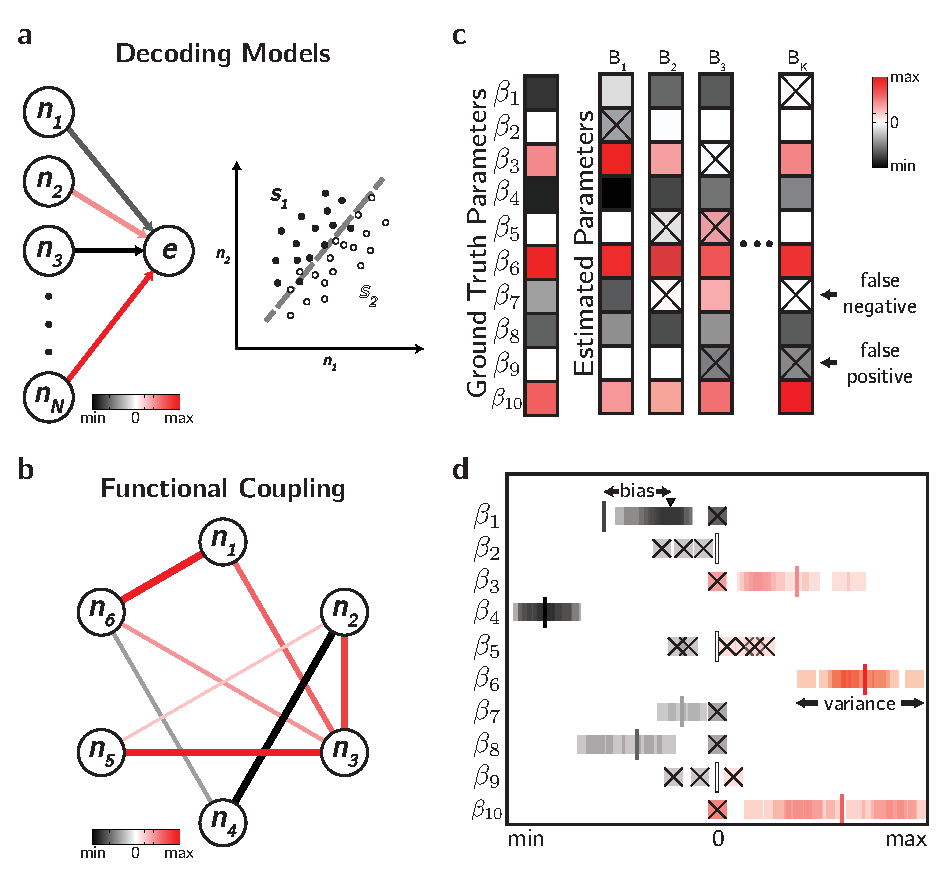
\includegraphics{./img/Fig1/Fig1}}
    \caption{\textbf{a} \textbf{b} Functional connectomics requires selecting and estimating non-zero edges. \textbf{c, d} Estimation of ground truth parameters over bootstraps of the data ($B_i$). Poor selection results in false positives and false negatives (\textbf{c}), while poor estimation results in high bias and high variance (\textbf{d}).}
    \label{fig:intro}
\end{figure}

We present the Union of Intersections (UoI) framework, a novel statistical approach we have recently introduced that addresses these issues \cite{uoi}. The algorithms enhanced by UoI (e.g., regression, classification, dimensionality reduction) are ubiquitous in systems neuroscience. Here, in real neuroscience analysis problems, we demonstrate qualitatively and quantitatively different results when using UoI-based methods compared to ``standard'' methods.  Thus, the foundational statistical improvements of UoI-based methods will potentially have significant impacts across neuroscience.
\section{METHODS}
UoI is not a single method or algorithm but a flexible statistical framework into which other algorithms (regression: Lasso; classification: Logistic Regression; dimensionality reduction: CUR/NMF; dynamics: Vector Autoregressive models) can be inserted. UoI-based methods leverage stochastic data resampling and a range of sparsity-inducing regularization parameters/dimensions to build families of potential feature sets robust to resamples (i.e., perturbations) of the data, and then average nearly unbiased parameter estimates of selected features to maximize predictive accuracy.

For concreteness, we consider an application of UoI in the context of linear regression. Specifically, we consider the problem of estimating the parameters $\beta \in \mathbb{R}^p$ that map a $p$-dimensional vector of predictor variables $x \in \mathbb{R}^p$ to the observation variable $y\in \mathbb{R}$, when there are $n$ paired samples of $x$ and $y$ corrupted by i.i.d Gausian noise:
$$
y = \beta^T x + \epsilon
$$
where $\epsilon \sim \mathcal{N}(0, \sigma^2)$ for each sample. When the true $\beta$ is thought to be sparse, an estimate of $\beta$ (i.e. $\hat{\beta}$) can be found by solving a constrained optimization problem of the form
$$
\hat{\beta} \in \underset{\beta\in \mathbb{R}^p}{\text{argmin}} \sum_{i=1}^n(y_i - \beta x_i)^2 + \lambda |\beta|_1
$$
where $|\beta|_1$ is the L1-norm of the parameters. Typically, $\lambda$ is unknown and must be determined through cross-validation across a variety of hyperparameters $\left\{\lambda_j\right\}_{j=1}^k$.

The key mathematical idea underlying UoI is to perform
model selection through intersection (compressive) operations and model estimation through union (expansive) operations, in that order. Thus, ``cross-validation'' is handled separately for selection and estimation. For UoI$_{\text{Lasso}}$, the procedure is as follows:
\begin{itemize}
    \item \textbf{Model Selection:} For each $\lambda_j$, generate Lasso estimates on $N_S$ resamples of the data. The selection profile $S_j$ (i.e. the set of non-zero parameters) for $\lambda_j$ consists of the features that persist in all model fits across the resamples (Fig. \ref{fig:uoi}, left).
    \item \textbf{Model Estimation:} For each unique support $S_j$, perform Ordinary Least Squares (OLS) on $N_E$ resamples of the data. The final model is obtained by averaging across the supports that optimally predict held-out data for each resample (Fig. \ref{fig:uoi}, right). 
\end{itemize}
Thus, the selection module ensures that, for each $\lambda_j$, only features that are stable to perturbations in the data (resamples) are allowed in the selection profile $S_j$. Meanwhile, the estimation module ensures that only the predictive selection profiles are averaged together in the final model. The degree of feature compression via intersections (quantified by $N_S$) and the degree of feature expansion via unions (quantified by $N_E$) can be balanced to maximize prediction accuracy of the sparsely estimated model parameters for the response variable $y$.
\begin{figure}[b]
    \centering
    \scalebox{0.50}{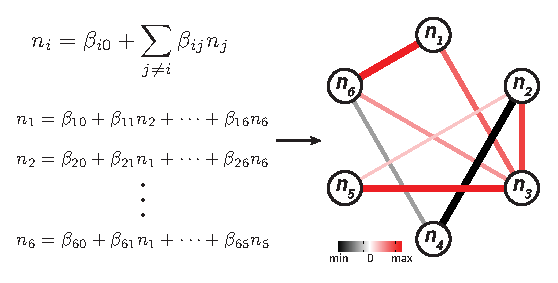
\includegraphics{./img/Fig2/Fig2}}
    \caption{The Union of Intersections framework applied to Lasso.}
    \label{fig:uoi}
\end{figure}
\section{RESULTS}
\subsection{Simulated Datasets}
To validate the performance of the UoI$_{\text{Lasso}}$ algorithm, we performed extensive numerical investigations on simulated data sets, where we controlled key properties of the data. We benchmarked UoI$_{\text{Lasso}}$ with five other selection/estimation methods: Ridge \cite{elements}, Lasso \cite{lasso}, Smoothly Clipped Absolute Deviation (SCAD) \cite{scad}, Boostrapped Adaptive Threshold Selection (BoATS) \cite{boats}, and debiased Lasso \cite{dbLasso}. 

We examined the performance of these algorithms across a variety of underlying distributions of model parameters, degrees of sparsity, and noise levels. Across all algorithms examined, we found that UoI$_{\text{Lasso}}$ (Fig. \ref{fig:simulated}, black) possessed: very high selection accuracy (Fig. \ref{fig:simulated}a); parameter estimates with low error, as quantified by $\text{RMS}=\sqrt{\frac{1}{p} \sum(\beta_i -\hat{\beta}_i)^2}$ (Fig. \ref{fig:simulated}b); the best prediction accuracy, quantified by $R^2$ (Fig. \ref{fig:simulated}c); and superior estimation variability as quantified by parameter variance, $E[\hat{\beta}^2] - E[\hat{\beta}]^2$ (Fig. \ref{fig:simulated}d). Additionally, UoI$_{\text{Lasso}}$'s high selection accuracy manifested as the most accurate model size (Fig. \ref{fig:simulated}e), which, in combination with its prediction accuracy, resulted in the best model parsimony as quantified by $\text{BIC} = -2\log \hat{\ell} + |\hat{\beta}_0| \log(n)$ (Fig. \ref{fig:simulated}f). Overall, UoI$_{\text{Lasso}}$ was robust to differences in underlying parameter distribution, degree of sparsity, and magnitude of noise.
\begin{figure}[t]
    \centering
    \scalebox{1.05}{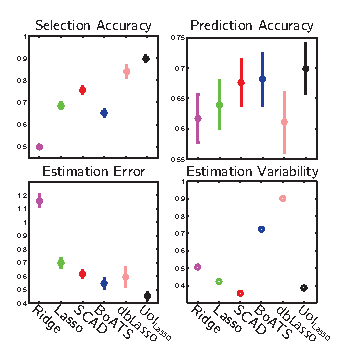
\includegraphics{./img/Fig3/Fig3}}
    \caption{Performance of UoI (black) compared to other models (in order: Ridge, Lasso, SCAD, BoATS, debiased Lasso) on simulated data.}
    \label{fig:simulated}
\end{figure}
\subsection{Sparse and Predictive Coupling Models from Non-human Primate Single-Unit Activity}
A significant strength of UoI$_{\text{Lasso}}$ is its ability to accurately deduce the true model size. Fig. \ref{fig:simulated}e revealed that several standard approaches have a propensity to exaggerate the model size (i.e. generate false positives). Thus, we examined whether, on a real dataset, UoI$_{\text{Lasso}}$ is able to extract more parsimonious models.

We considered single-unit spiking activity from primary motor cortex (M1) of Macaque monkey during self-paced reaches on a grid ($p=196$ single-units) \cite{nhp}. We binned the spike counts at 500 milliseconds and applied a square-root transform to stabilize the variance (resulting in $n=1716$ samples). Then, for each neuron $i$, we predicted the stabilized spike counts $y_i$ using the activities of the remaining neurons,
$$
y_i = \beta_{i0} + \sum_{j\neq i} \beta_{ij} y_j.
$$
The fitted parameters $\beta_{ij}$ detail the coupling structure for the population of neurons.

We compared the coupling fits generated by Lasso and UoI$_{\text{Lasso}}$ for each of the 196 units. UoI$_{\text{Lasso}}$ provided considerably sparser fits, as quantified by the selection ratio (fraction of non-zero features: Fig. \ref{fig:nhp}, top-left). On average, UoI$_{\text{Lasso}}$ used 8 times fewer parameters than Lasso. However, UoI$_{\text{Lasso}}$ maintained the predictive quality across all the fits (Fig. \ref{fig:nhp}, top-right). These two observations can be summarized succinctly with the Bayesian Information Criterion (BIC), a metric for model parsimony. The difference in BIC $(\Delta$BIC = BIC$_{\text{Lasso}}-$BIC$_{\text{UoI}})$ across the model fits is shown in Fig. \ref{fig:nhp}, bottom. About a quarter of the fits exhibit little to no difference in BIC, indicating there is little evidence against the models provide by Lasso.  Meanwhile, about 70\% of the single-units have a difference in BIC of at least 10, indicating very strong evidence against Lasso as a descriptive model of the data \cite{kass1995}. Thus, UoI$_{\text{Lasso}}$ provides coupling models that are as simple as possible, but no simpler. 
\begin{figure}[t]
    \centering
    \scalebox{0.55}{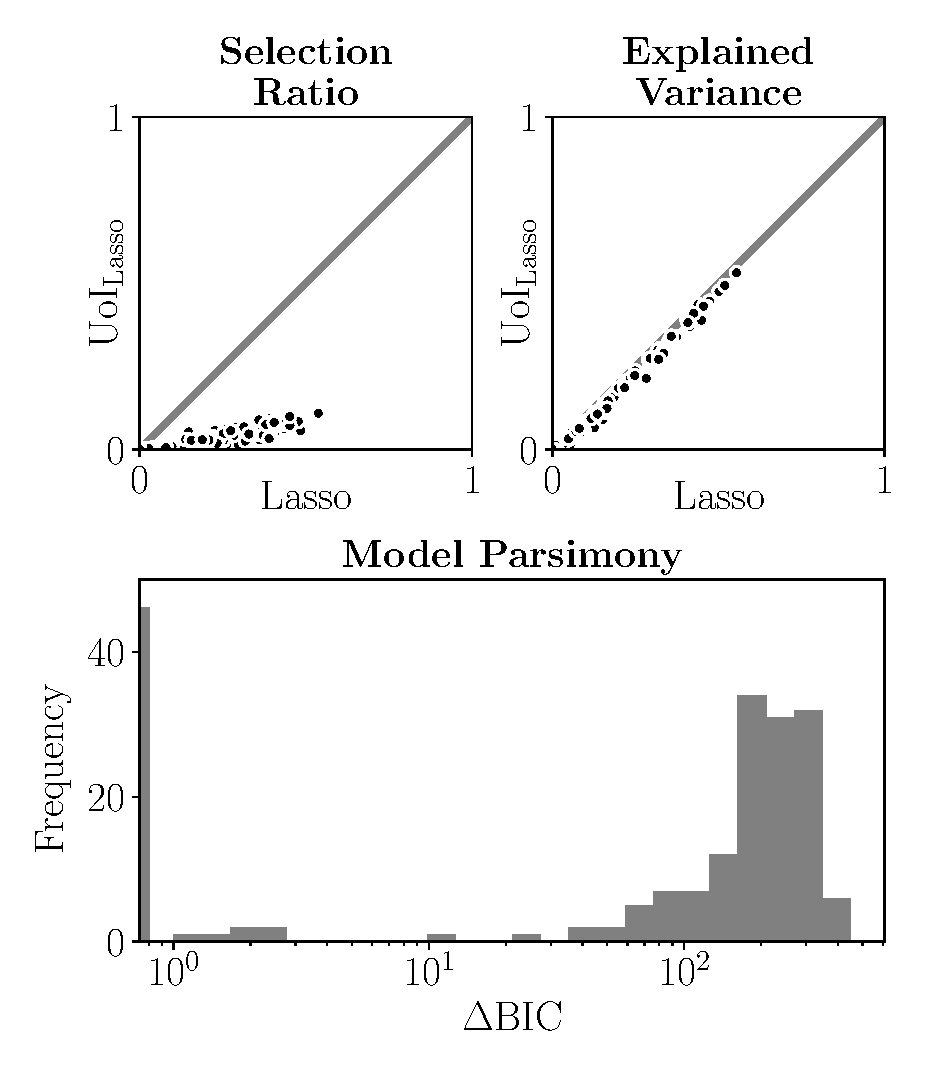
\includegraphics{./img/Fig5/Fig5}}
    \caption{UoI$_{\text{Lasso}}$ generates more parsimonious coupling models of spiking data. Top left: Comparison of selection ratios (fraction of non-zero features) for each coupling fit. Each point represents one single-unit. Top right: Comparison of $R^2$ values for each coupling fit. Bottom: Difference in BIC between Lasso and UoI$_{\text{Lasso}}$.}
    \label{fig:nhp}
\end{figure}
\subsection{Sparse Functional Networks from Human Neural Recordings}

We sought to determine if the enhanced selection and estimation properties of UoI$_{\text{Lasso}}$ also improved its utility as a tool for data-driven discovery in complex, diverse neuroscience data sets. Thus, we tackled the problem of graph formation from multi-electrode ($p=86$ electrodes) neural recordings taken directly from the surface of the human brain during speech production ($n=45$ trials each) \cite{bouchard2013}. That is, the goal was to construct sparse neuroscientifically-meaningful graphs for further downstream analysis. To estimate functional connectivity, we calculated partial correlation graphs. The model was estimated independently for each electrode, and we compared the results of graphs estimated by UoI$_{\text{Lasso}}$ to the graphs estimated by SCAD. In Fig. \ref{fig:vsmc}a-b, we display the networks derived from recordings during the production of /b/ while speaking /ba/. We found that the UoI$_{\text{Lasso}}$ network (Fig. \ref{fig:vsmc}a) was much sparser than the SCAD network (Fig. \ref{fig:vsmc}b). Furthermore, the network extracted by UoI$_{\text{Lasso}}$ contained electrodes in the lip (dorsal vSMC), jaw (central vSMC), and larynx (ventral vSMC) regions, accurately reflecting the articulators engaged in the production of /b/ (Fig. \ref{fig:vsmc}c). The SCAD network (Fig. \ref{fig:vsmc}d) did not have any of these properties. This highlights the improved power of UoI$_{\text{Lasso}}$ to extract sparse graphs with functionally meaningful features relative to even some non-convex methods.
\begin{figure}[t!]
    \centering
    \scalebox{0.75}{\includegraphics{./img/Fig4/Fig4}}
    \caption{\textbf{a, b} Partial correlation graphs obtained from UoI$_{\text{Lasso}}$ and SCAD, respectively. \textbf{c, d} The locations of the electrodes on vSMC. \textbf{e} Average relative prediction accuracy (compared to baseline) during the production of a consonant-vowel syllable. \textbf{f} Average selection ratio over the same time course.}
    \label{fig:vsmc}
\end{figure}

We calculated connectivity graphs during the production of 9 consonant-vowel syllables. Fig. \ref{fig:vsmc}e displays a summary of prediction accuracy for UoI$_{\text{Lasso}}$ networks (red) and SCAD networks (black) as a function of time. The average relative prediction accuracy (compared to baseline times) for the UoI$_{\text{Lasso}}$ network was generally greater during the time of peak phoneme encoding ($T = \left[-100:200\right]$) compared to the SCAD network. Fig. \ref{fig:vsmc}f plots the time course of the parameter selection ratio for the UoI$_{\text{Lasso}}$ network (red) and SCAD network (black). The UoI$_{\text{Lasso}}$ network was consistently $\sim5$ times sparser than the SCAD network. These results demonstrate that UoI$_{\text{Lasso}}$ extracts sparser graphs from noisy neural signals with a modest increase in prediction accuracy compared to SCAD.

\section{CONCLUSION}

UoI-based methods leverage stochastic data resampling and a range of sparsity-inducing regularization parameters/dimensions to build families of potential features, and then average nearly unbiased parameter estimates of selected features to maximize predictive accuracy. Thus, UoI separates model selection with intersection operations from model estimation with union operations: the limitations of selection by intersection are counteracted by the union of estimates, and vice versa. Stochastic data resampling can be a viewed as a perturbation of the data, and UoI efficiently identifies and robustly estimates features that are stable to these perturbations. Here, we demonstrated that these properties result in both superior selection and estimation performance on simulated data as well as the generation of sparse, interpretable models on neuroscience datasets.

In this work, we focused on neuroscience applications of UoI$_{\text{Lasso}}$. However, other machine learning algorithms fit naturally in the UoI framework. For example, we have successfully developed  the UoI$_{\text{Logistic}}$, UoI$_{\text{Poisson}}$, UoI$_{\text{VAR}}$, UoI$_{\text{CUR}}$, and UoI$_{\text{NMF}}$ algorithms and applied them to neuroscience datasets. In addition, UoI has a high degree of natural algorithmic parallelism that we have exploited in a distributed Python-MPI implementation. With the diversity of use cases and ease of application to large datasets, UoI has the potential to provide data-driven insight in a variety of neuroscientific and biomedical contexts.

\addtolength{\textheight}{-12cm}   % This command serves to balance the column lengths
                                  % on the last page of the document manually. It shortens
                                  % the textheight of the last page by a suitable amount.
                                  % This command does not take effect until the next page
                                  % so it should come on the page before the last. Make
                                  % sure that you do not shorten the textheight too much.

%%%%%%%%%%%%%%%%%%%%%%%%%%%%%%%%%%%%%%%%%%%%%%%%%%%%%%%%%%%%%%%%%%%%%%%%%%%%%%%%



%%%%%%%%%%%%%%%%%%%%%%%%%%%%%%%%%%%%%%%%%%%%%%%%%%%%%%%%%%%%%%%%%%%%%%%%%%%%%%%%



%%%%%%%%%%%%%%%%%%%%%%%%%%%%%%%%%%%%%%%%%%%%%%%%%%%%%%%%%%%%%%%%%%%%%%%%%%%%%%%%

\section*{ACKNOWLEDGMENT}

P.S. Sachdeva was supported by the Department of Defense (DoD) through the National Defense Science \& Engineering Graduate Fellowship (NDSEG) Program.


%%%%%%%%%%%%%%%%%%%%%%%%%%%%%%%%%%%%%%%%%%%%%%%%%%%%%%%%%%%%%%%%%%%%%%%%%%%%%%%%




\begin{thebibliography}{99}

\bibitem{uoi} K. E. Bouchard, A. F. Bujan, F. Roosta-Khorasani, S. Ubaru, Prabhat, A. M. Snijders, J.-H. Mao, E. F. Chang, M. W. Mahoney, and S. Bhattacharyya. Union of Intersections (UoI) for interpretable data driven discovery and prediction, In \textit{Annual Advances in Neural Information Processing Systems, 30: Proceedings of the 2017 Conference}, 2017.
\bibitem{elements} T. Hastie, R. Tibshirani, and J. Friedman, The Elements of Statistical Learning. Springer-Verlag, New York, 2003.

\bibitem{lasso} R. Tibshirani, Regression shrinkage and selection via the lasso, \textit{Journal of the Royal Statistical Society: Series B}, vol. 58, no. 1, pp. 267-–288, 1996.

\bibitem{scad} J. Fan and R. Li, Variable selection via nonconcave penalized likelihood and its oracle properties, Journal of the American Statistical Association, vol. 96 no. 456, pp. 1348–-1360, 2001.

\bibitem{boats} K. E. Bouchard, Bootstrapped adaptive threshold selection for statistical model selection and estimation, arXiv:1505.03511, 2015.

\bibitem{dbLasso} A. Javanmard and A. Montanari, Confidence intervals and hypothesis testing for high-dimensional regression, Journal of Machine Learning Research, vol. 15, pp. 2869–-2909, 2014.

\bibitem{nhp} J. E. O'Doherty, M. M. B. Cardoso, J. G. Makin, and P. N. Sabes, Nonhuman Primate Reaching with Multichannel Sensorimotor Cortex Electrophysiology [Data set], Zenodo, 2017.

\bibitem{bouchard2013} K. E. Bouchard, N. Mesgarani, K. Johnson, and E. F. Chang, Functional organization of human sensorimotor cortex for speech articulation, \textit{Nature}, vol. 495, no. 7441, pp. 327–-332, 2013.

\bibitem{kass1995} R. E. Kass and A. E. Raftery, Bayes Factors, \textit{Journal of the American Statistical Association}, vol. 90, no. 430, pp. 773-–795, 1995.






\end{thebibliography}




\end{document}
